\documentclass{article}
\usepackage[margin=1in]{geometry}
\usepackage{amsmath}
\usepackage{amssymb}
\usepackage{booktabs}
\usepackage{float}
\usepackage{graphicx}
\usepackage{hyperref}
\usepackage{pdfpages}
\usepackage{siunitx}
\usepackage{adjustbox}
\usepackage{cancel}
\usepackage{paracol}
\usepackage{placeins}

\usepackage{parskip}

\globalcounter{figure}
\counterwithin{equation}{section}

\title{Report}
\date{16 March 2026}
\author{Connor Emmons}

\begin{document}
\pagenumbering{gobble}
\maketitle
\vfill
\paragraph*{Notes}

\newpage
\pagenumbering{arabic}

\section{First Attempt at Generating Cyclers with Z-Components}

For a first attempt, remove the bound on the initial and final z velocity being zero, and simply take the good 3D orbit and rotate it by 45 degrees about the x-axis for the initial guess. This just generated the solution where the spacecraft does a quick burn to just stay still.

For the next attempt, drop the weights of the Jacobi constant and the final Jacobi constant to 0.5, and keep the weight on the control at 1. The thought is to force less control and try to minimize the Jacobi error (the Jacobi is still for the planar orbit though). With these, the solution given is just the planar solution. Upon further mathematical investigation, the Jacobi constant is correct.

Dropping the weights off of the Jacobi constant terms (just minimizing control) gives a potentially feasible orbit, but it is planar.

\begin{figure}[H]
    \centering
    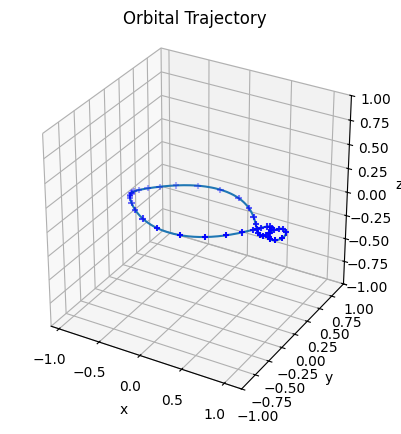
\includegraphics[width=\columnwidth]{planar1.png}
    \caption{Planar Orbit, valid according to Jacobi and Hamiltonian}
\end{figure}

Next, try to force the orbit angle. Minimize:

\begin{equation}
    W_{cf}\left(C_f - C_f*\right)^2 + \int{W_c(C - C*)^2 + W_u\left(u_x^2 + u_y^2 + u_z^2\right) + W_{\theta}\left(\left|\arctan\frac{z}{y}\right| - \theta_{desired}\right)^2}
\end{equation}

Begin by keeping Jacobi weights at zero and use initial guess tilted by 45 degrees.

Broke because when z and y are both zero, arctan function breaks. Instead, use velocity (Nope, broke because you used \^{} instead of **). Thus, minimize:

\begin{equation}
    W_{cf}\left(C_f - C_f*\right)^2 + \int{W_c(C - C*)^2 + W_u\left(u_x^2 + u_y^2 + u_z^2\right) + W_{\theta}\left(\mod\left(\arctan2\frac{vz}{vy}, \pi\right) - \theta_{desired}\right)^2}
\end{equation}

This ran for 8 minutes only to find the null solution. Next, try to run with position instead of velocity now that the error is fixed.

4 minutes to generate the null solution. Add back in Jacobi constant weights at 0.5. Took 23 minutes to find the null solution. Drop the tolerance to 1e-20 and try just weighting the final Jacobi constant with 10.

15 minutes to generate the null solution. Try setting a lower bound on the final time at 1. This produced the spaghetti monster.

\begin{figure}[H]
    \centering
    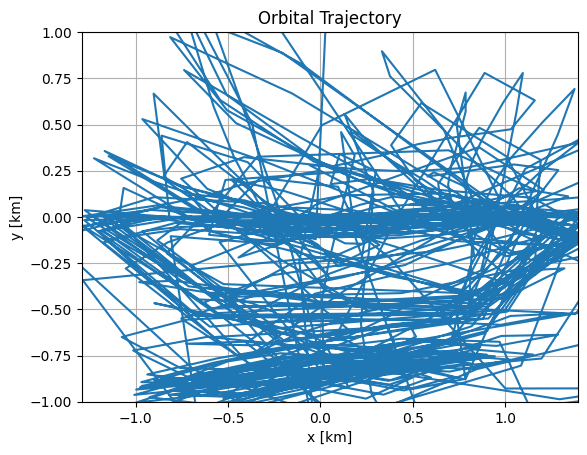
\includegraphics[width=\columnwidth]{spaghetti1.png}
    \caption{Useless}
\end{figure}

\begin{figure}[H]
    \centering
    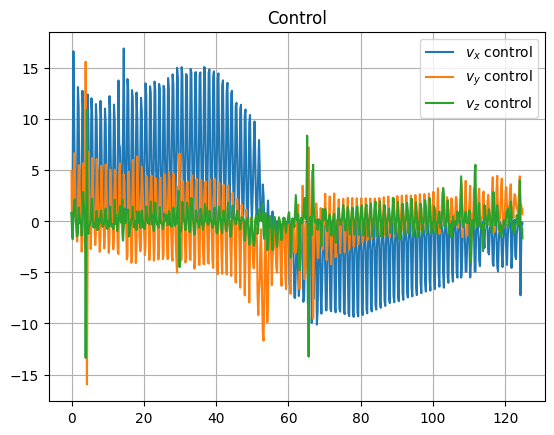
\includegraphics[width=\columnwidth]{spaghetticontrol.png}
    \caption{Control for spaghetti}
\end{figure}

Next, try bounding the controls at 1. This took 25 minutes to generate a potentially good orbit.

\begin{figure}[H]
    \centering
    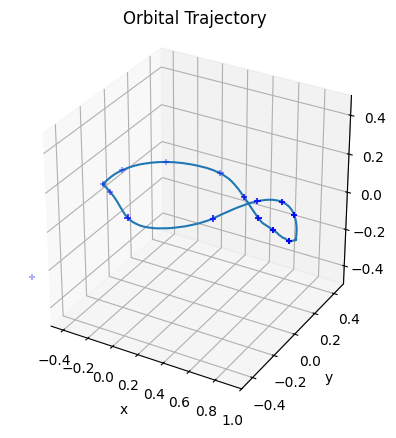
\includegraphics[width=\columnwidth]{potential1.png}
    \caption{Potential Orbit}
\end{figure}

\begin{figure}[H]
    \centering
    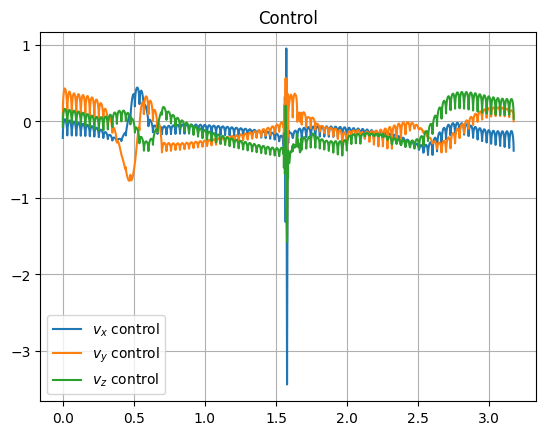
\includegraphics[width=\columnwidth]{potentialcontrol.png}
    \caption{Control for Potential Orbit}
\end{figure}

\begin{figure}[H]
    \centering
    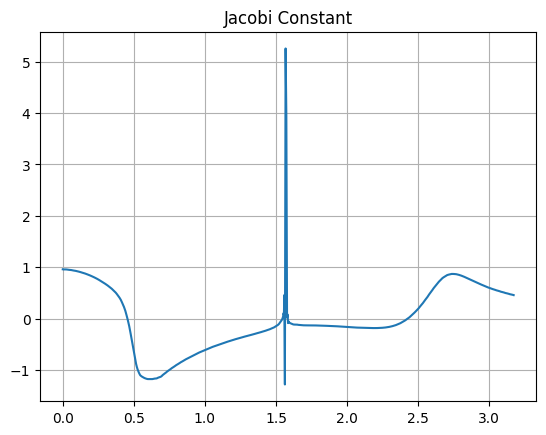
\includegraphics[width=\columnwidth]{potentialjacobi.png}
    \caption{Jacobi for Potential Orbit}
\end{figure}

\begin{figure}[H]
    \centering
    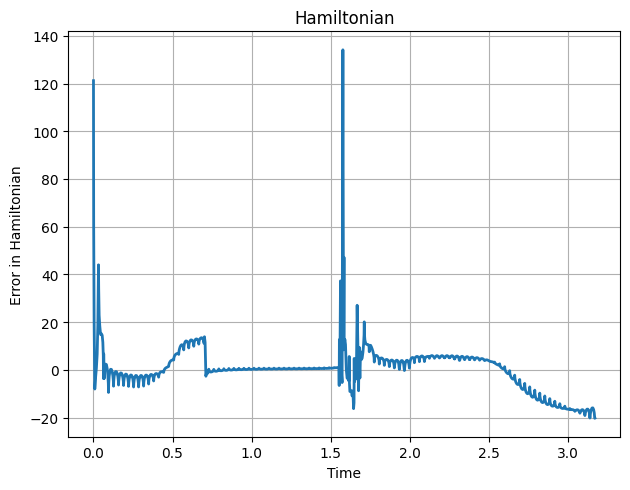
\includegraphics[width=\columnwidth]{potentialhamiltonian.png}
    \caption{Hamiltonian for Potential Orbit}
\end{figure}

Next, try to find an orbit that's more ballistic. Drop the weighting on the final jacobi constant to 5, increase the weighting on the control to 5, and drop the weighting on the angle to 0.5. Additionally, set the lower bound on control to -1.

Result is not very ballistic, but Hamiltonian is promising - this might actually be a feasible orbit.

\begin{figure}[H]
    \centering
    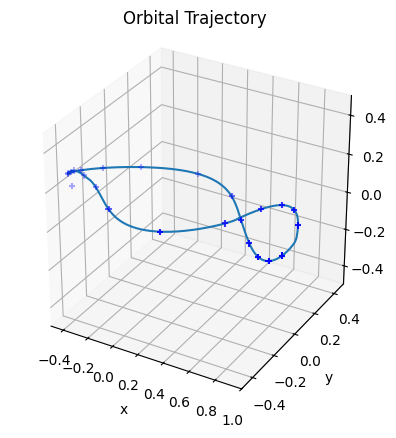
\includegraphics[width=\columnwidth]{potential2.png}
    \caption{An actually maybe good orbit}
\end{figure}

\begin{figure}[H]
    \centering
    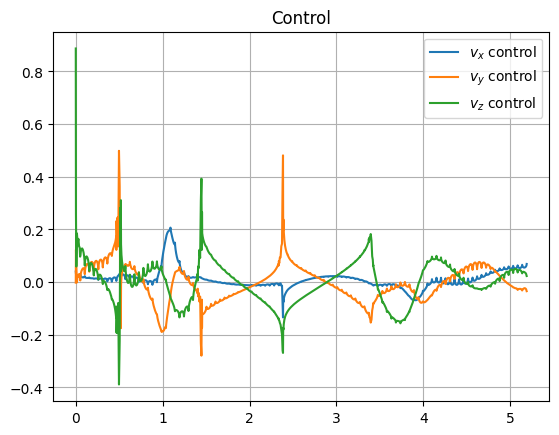
\includegraphics[width=\columnwidth]{potenetial2control.png}
    \caption{Control}
\end{figure}

\begin{figure}[H]
    \centering
    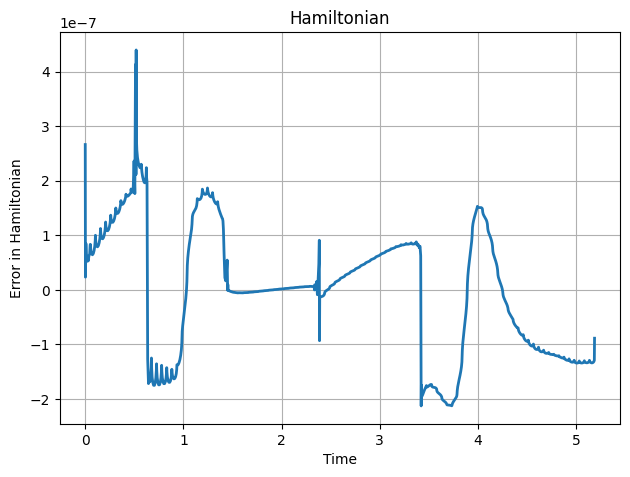
\includegraphics[width=\columnwidth]{potential2hamiltonian.png}
    \caption{Hamiltonian}
\end{figure}

Fix the lower bound issue that existed for the first run with final Jacobi at 10, control at 1, and angle at 1. This produced an orbit that may be plausible, but the Hamiltonian says that this is unlikely.

\begin{figure}[H]
    \centering
    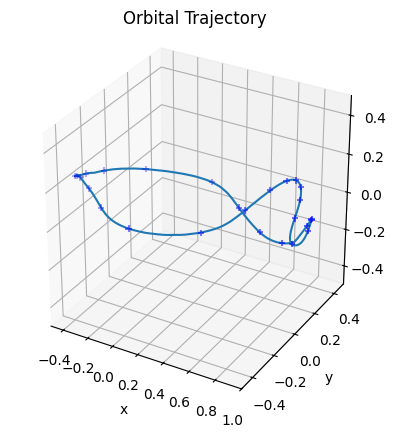
\includegraphics[width=\columnwidth]{potential3.png}
    \caption{Potential Orbit, but Hamiltonian is no good}
\end{figure}

\begin{figure}[H]
    \centering
    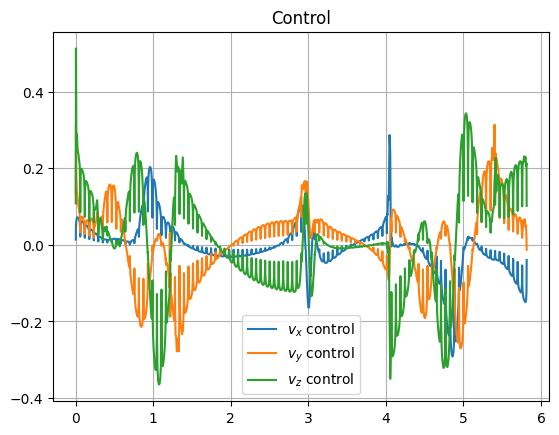
\includegraphics[width=\columnwidth]{control3.png}
    \caption{Control}
\end{figure}

\begin{figure}[H]
    \centering
    
\includegraphics[width=\columnwidth]{hamiltonian3.png}
    \caption{Hamiltonian}
\end{figure}

\end{document}